\documentclass{article}
\usepackage{graphicx}
\graphicspath{{images/}}

\title{
    User Manual\\
    \begin{large}
        \textit{Golf Course Mapper}
    \end{large}
}
\date{
    \begin{small}
        \today
    \end{small}
}
\author{
    Team Recursive Recursion \\
    Retro Rabbit
}

\begin{document}
    %===========================================================================
    % TITLE
    %===========================================================================
    \pagenumbering{gobble}
    \maketitle
    \newpage

    %===========================================================================
    % DOCUMENT
    %===========================================================================
    \pagenumbering{arabic}

    
    \tableofcontents
    \newpage
	\section{System Overview}    
	\paragraph{}
	The goal of the project is to allow golf course owners/managers to draw the shape of their
courses using a web application. Details such as the location of the hole and any natural
hazards can also be included in the map of the course.

Players on the course are then able to use a mobile application to see the map of the
course and their location on it. This will allow the players to plan their shots more
strategically. Additionally, the managers will be able to view the live location of any
active players.


	\section{System Configuration}
	 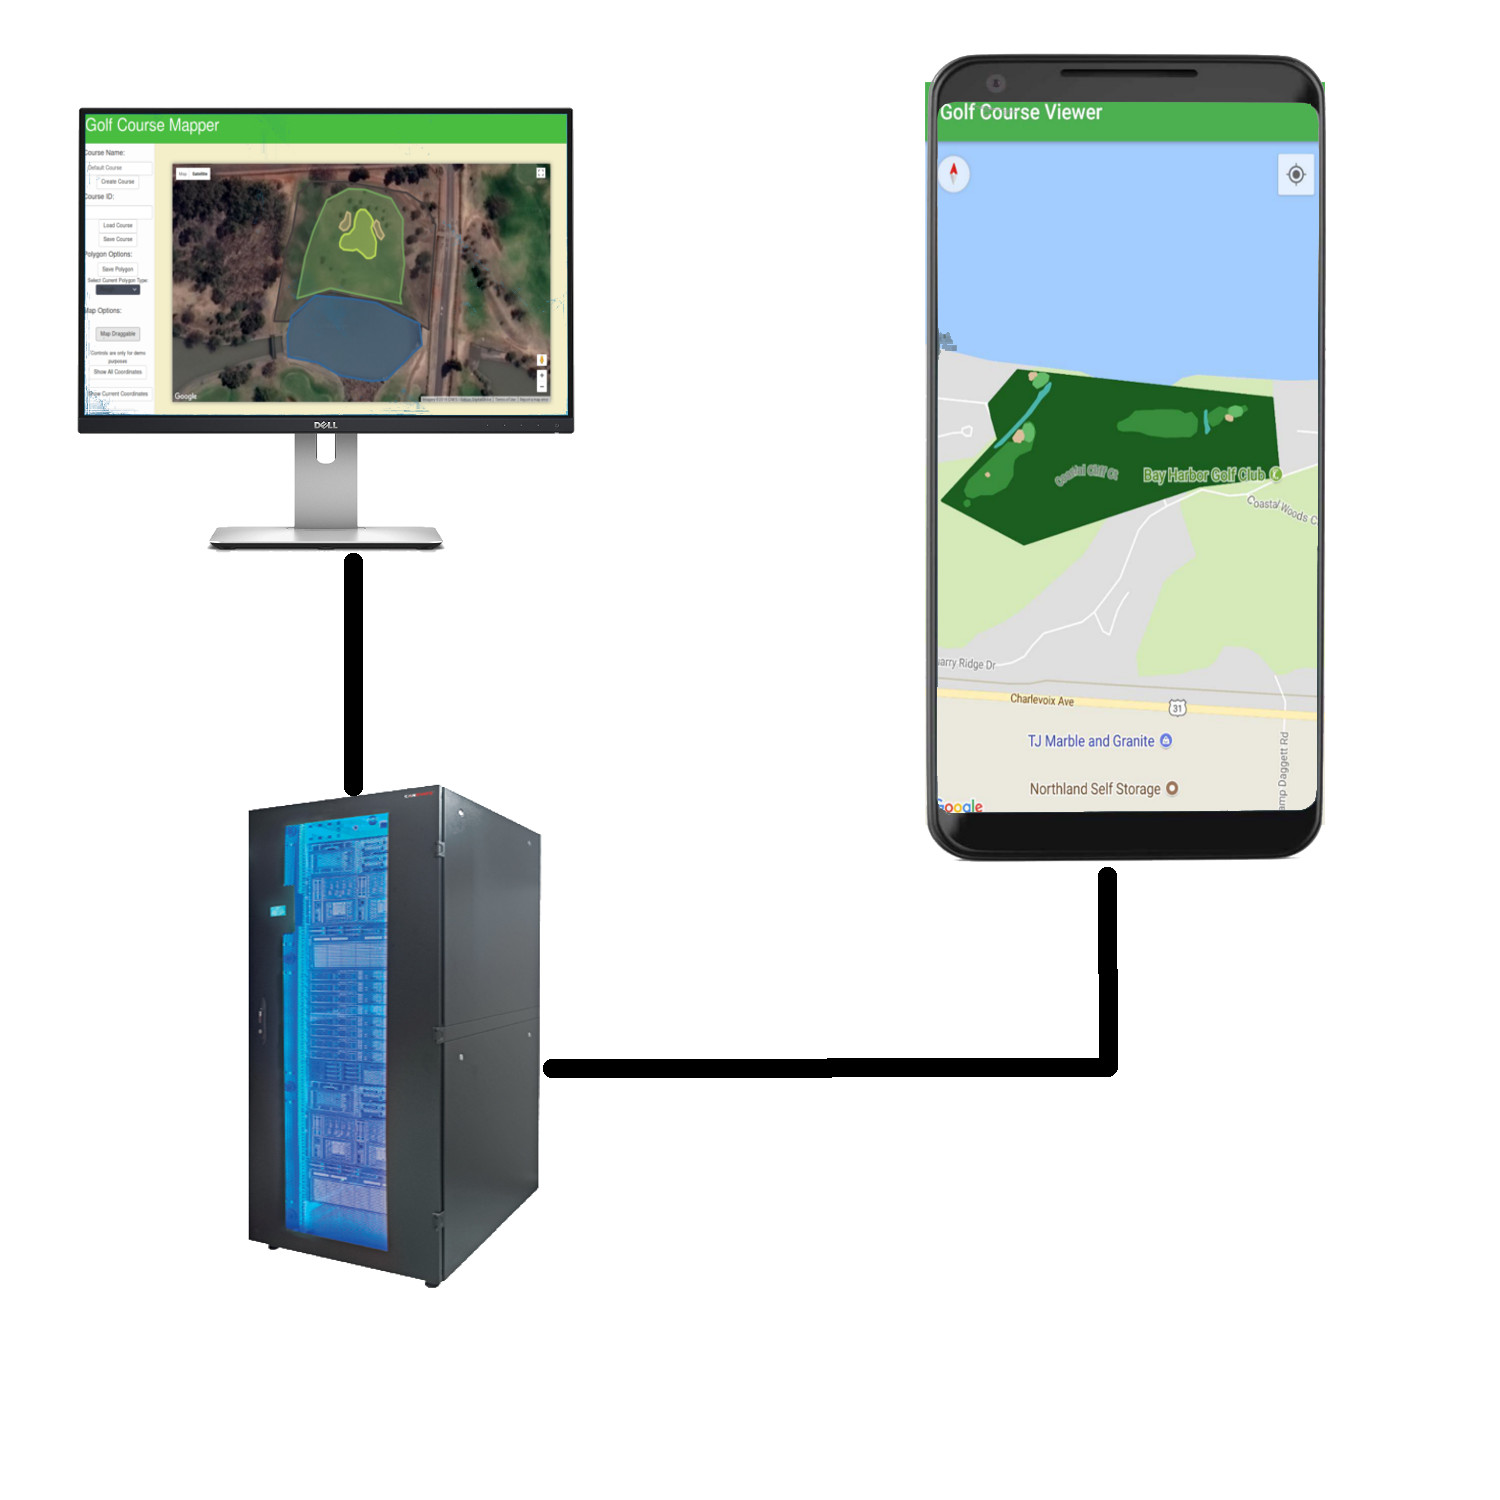
\includegraphics[scale=0.25]{sys-conf-diagram.jpg}
	\paragraph{•}
	  The website and the mobile application connects to the server to retrieve data. An Internet connection is needed to load the map on both the web and mobile application. It is recommended to have Android 4.4 or later for the mobile application. The latest version of Internet Explorer, Google Chrome or Mozilla Firefox is recommended.
	  
	  \section{Installation}
	
	  \paragraph{•}
	  Website: The website is installed on a server but the source code can be found on github.
	  Mobile App: The app can be found on the Google Play store, just click on the install button and launch the application. \linebreak https://play.google.com/store/apps/details?id=recrec.golfcourseviewer
	
	\section{Getting Started}
	\paragraph{•}
	
	Website: To access the website go to the URL (http://ec2-18-191-152-232.us-east-2.compute.amazonaws.com).If this is your first time using the website, please register your credentials. If you have used the website before login with your credential that you used to register. 
	
	Mobile Application: To access the mobile application press on the application on a mobile device to launch the application.
	\section{Using the System}
	
	\subsection{Website}
	\paragraph{•}
	When you go to the website (http://ec2-18-191-152-232.us-east-2.compute.amazonaws.com) 			     you will greeted by the homepage as seen in figure 1 below.	
	
	
	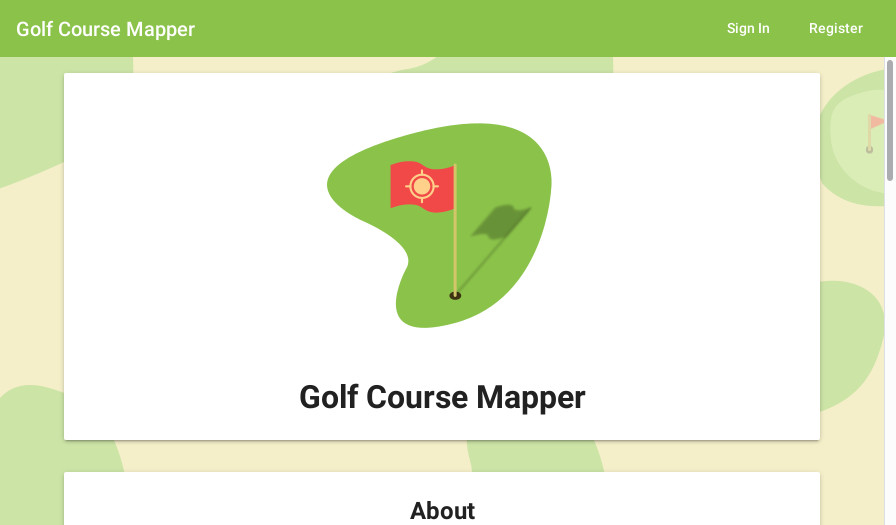
\includegraphics[scale=1.2]{0_home}
	\paragraph{•}
    Figure 1.
	
	
	\subsubsection{Register}
	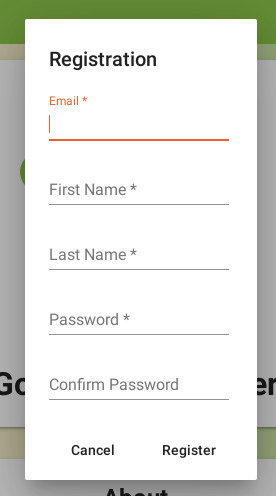
\includegraphics[scale=1.5]{1_register}
	\paragraph{•}
    Figure 2.
	\paragraph{•}
	The first time you use the website you must register. You can't use the website without registering. To register for the website, type in your credentials in the text boxes as seen in figure 2. The following details must be entered:
	
	\begin{itemize}
		\item Email
		\item First Name
		\item Last Name
		\item Password
		\item Confirm Password
	\end{itemize}
	
	
	\paragraph{•}
	You must type your password twice to ensure they are the same.After your details have been 	entered, click on the Register button to register. A message will show that you successfully registered and can now use the website. If you receive an error, see the troubleshooting section.
	
		
	
	
	\subsubsection{Login}
	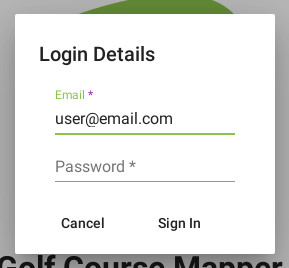
\includegraphics[scale=1.5]{2_login}
	\paragraph{•}
    Figure 3.
	\paragraph{•}
	After you have successfully registered, you can now login. Type in the same Email and Password that you registered with, click on the Login button to login. As seen in figure 3. If the details are correct, you will be logged in. You will now be logged in and you can now use the website to map a golf course. You will be greeted by a map of the world.	
   
    
	\subsubsection{Select a Golf Course}
	 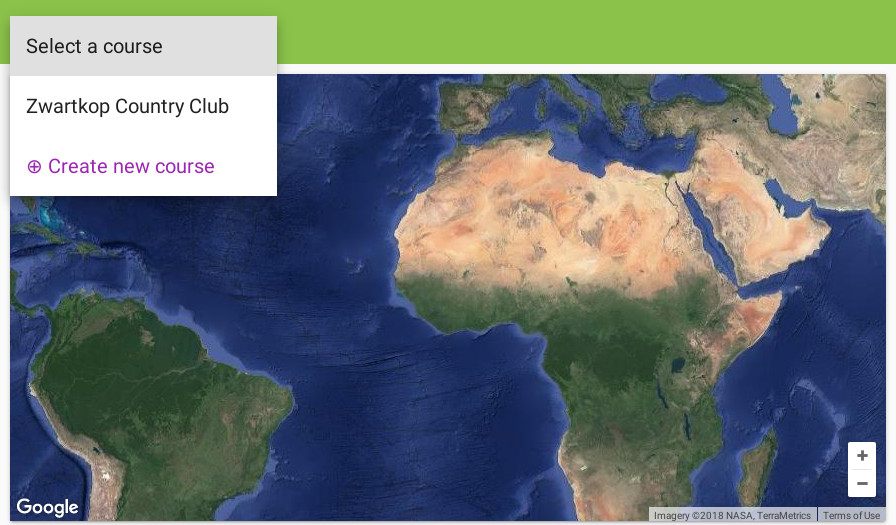
\includegraphics[scale=1.5]{3_create_course}
	\paragraph{•}
    Figure 4.    
	\paragraph{•}    
	If you would like to load a previous golf course. Click on the "Select a course" text as shown in Figure 4. A drop down menu will appear with all the available course. Click on the name desired course to load the course onto the map. You would want to do this if you want to load and edit a previous course.
    
    \subsubsection{Select a Golf Course}
	 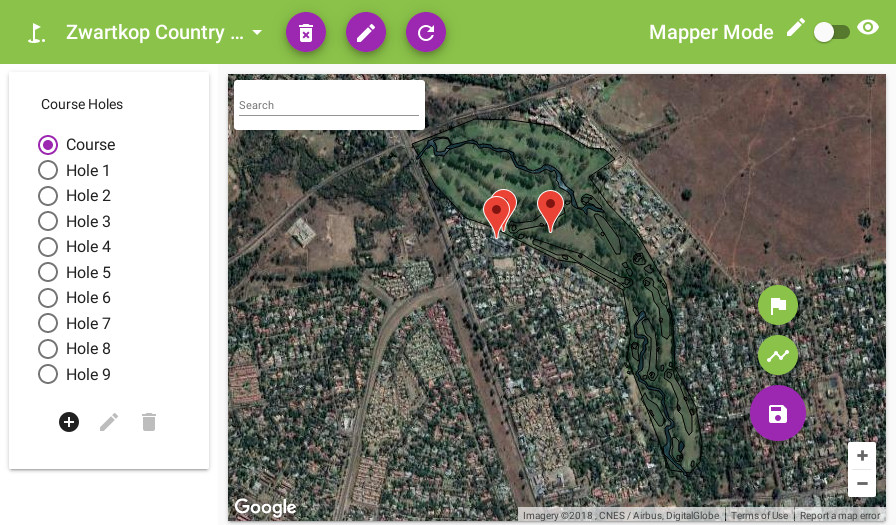
\includegraphics[scale=1.5]{5_selected}
	 \paragraph{•}
    Figure 5.  
	 
	 \paragraph{•}
	 After you selected a course, you will be shown the course on the map as seen in Figure 5 above.
    
    \subsubsection{Create Golf Course}
    \paragraph{•}
    To create a new golf course, click on the "Create new course" as seen in Figure 4 above. After you clicked on the "Create new course" a new window will appear, as seen in Figure 6. Type in the following details on the course:
    
    \begin{itemize}
    		\item Golf course name
    		\item Optional info about the golf course
    \end{itemize}
    
    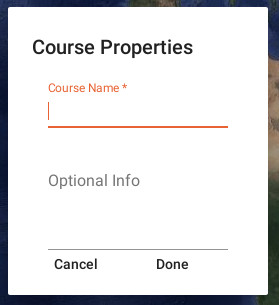
\includegraphics[scale=1.5]{4_create_course_popup}
	\paragraph{•}
    Figure 6.
	
    
    \subsubsection{Create a Hole}
    \paragraph{•}
     Click on the "+" icon on the left to create a new hole. Use this option when you want to add another golfhole to the golfcourse. In Figure 6 the new window is shown. The following details must be typed in for the hole.
     
     \begin{itemize}
    		\item Hole name
    		\item Par of the hole
    \end{itemize}
    
    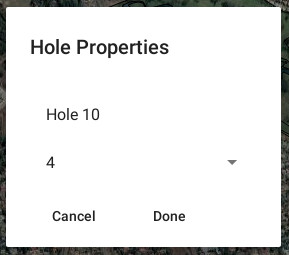
\includegraphics[scale=1.5]{6_hole_popup}
	\paragraph{•}
    Figure 7.
    
    \subsubsection{Mapper Mode}
    
\includegraphics[scale=1.5]{7_mapper_mode}
	\paragraph{•}
    Figure 8.
    
    \paragraph{•}
    To change between viewing and editing mode, click on the toggle button as shown in Figure 8. The edit mode is on the left (the pencil) and the view mode is on the right (the eye). You can edit a golfcourse when it is in edit mode and see live locations when it is view mode.
    
    \subsubsection{Delete an Element}
    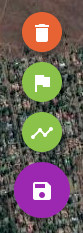
\includegraphics[scale=1.5]{8_map_controls}
	\paragraph{•}
    Figure 9.
    \paragraph{•}
    To delete an element click on the element and then click on the red trash can icon. The selected element will now be deleted. Use this option when you placed an element incorrectly and want to remove/delete it. As seen in Figure 8 above.
    
    \subsubsection{Place a Marker}
	\paragraph{•}
	To place a marker on the map, click on the green flag icon on the right of the screen as seen in Figure 8. Click on a desired location for the marker to be placed. A menu will appear to select the type of marker and to add additional information. Click on the done button to finish the marker placing. The available markers are:
	
	\begin{itemize}
	\item Hole
	\item Tee
	\item Pin
	\end{itemize}
	

    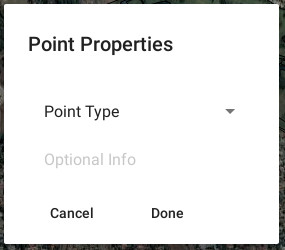
\includegraphics[scale=1.5]{11_point}
	
	\subsubsection{Create Area}
    \paragraph{}
    To create a polygon or map out a element, click on the green line icon as seen in Figure 8. To create the polygon click on the map in the desired locations. Lines will appear as the user click, when the polygon has been completed a menu will appear to choose the element type. The available types are: 
    
    \begin{itemize}
     \item Green
     \item Fairway
     \item Water hazard
     \item Sand Bunker
    \end{itemize}
    
    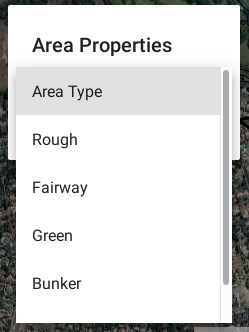
\includegraphics[scale=1.5]{10_area}
    
     \subsubsection{Save Course} 
    \paragraph{}
    To save changes made to a course or hole, click on the purple save icon on the right of the screen. Any changes made will now be saved. As shown in figure 8.
    
	\subsubsection{Reload Course}   
	
\includegraphics[scale=1.5]{9_course_controls} 
	Figure 10
	\paragraph{•}
	To reload the course, click on the purple reload icon on the screen as shown above. The map will now reload.
	
    \subsubsection{Delete Course}
	\paragraph{•} 
	To delete a course, load the desired course. Click on the purple trash can on the right of the course name to delete the golf course. As seen above at Figure 10.


	\subsection{Mobile Application}
	    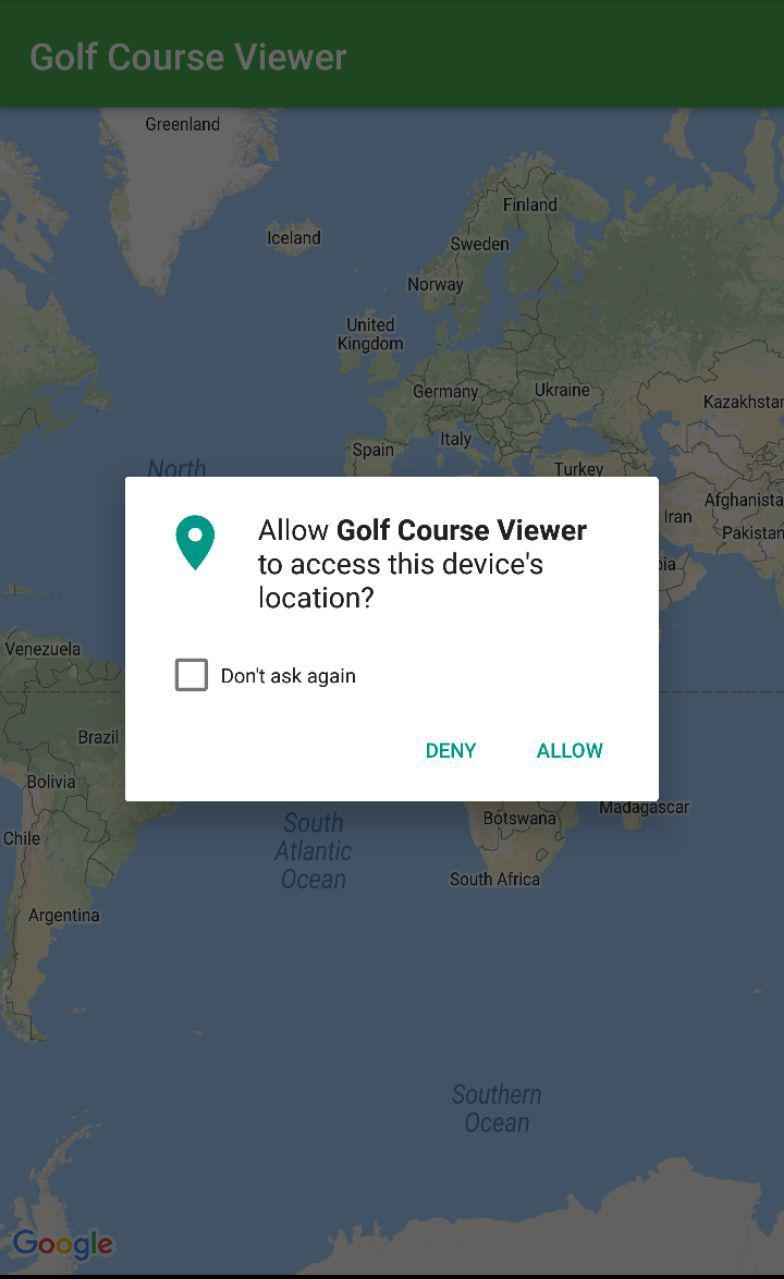
\includegraphics[scale=0.2]{mobileapp-permissions.jpg}
	    \linebreak
	    Figure 11
	\subsubsection{Allow Permissions}
	
	\paragraph{•}
	When starting the application, a message will pop up to ask for permissions to use location services. Press "Allow" to allow location services to be used. This is necessary to find your current location so that you can see how far you are from points of interest.
	
	\subsubsection{View Course}
	    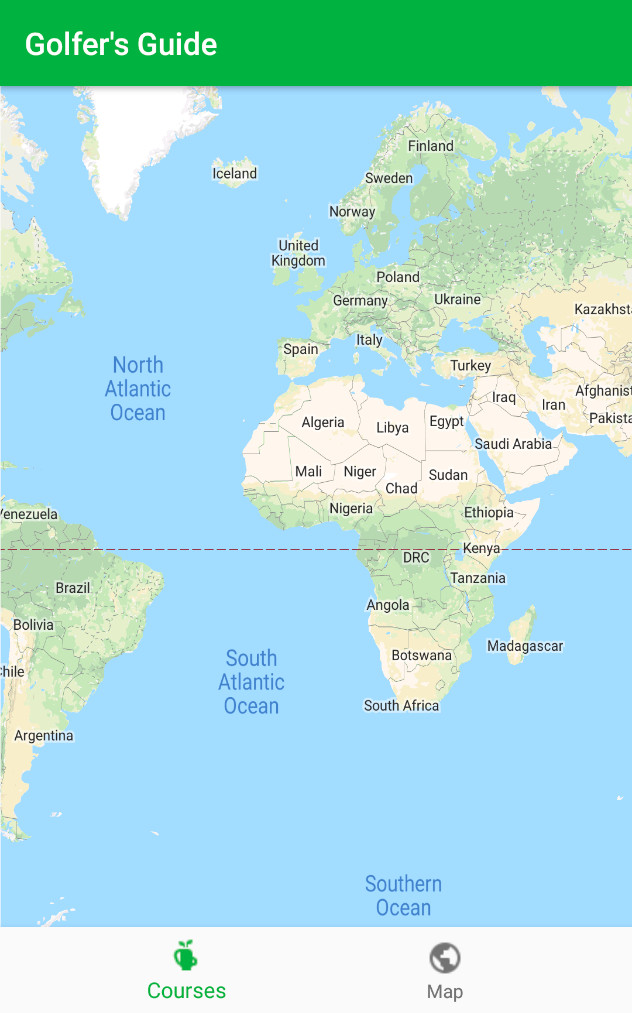
\includegraphics[scale=0.8]{0_overview}
	    Figure 12
	
	\paragraph{•}
	You will be shown this screen when you launch the app. Move around by touching and zoom by pinching the screen. Move to the location of gold course created to view the course. The next hole can be seen by tapping on the blue arrow on the right button
	
	\subsubsection{Select Course}
	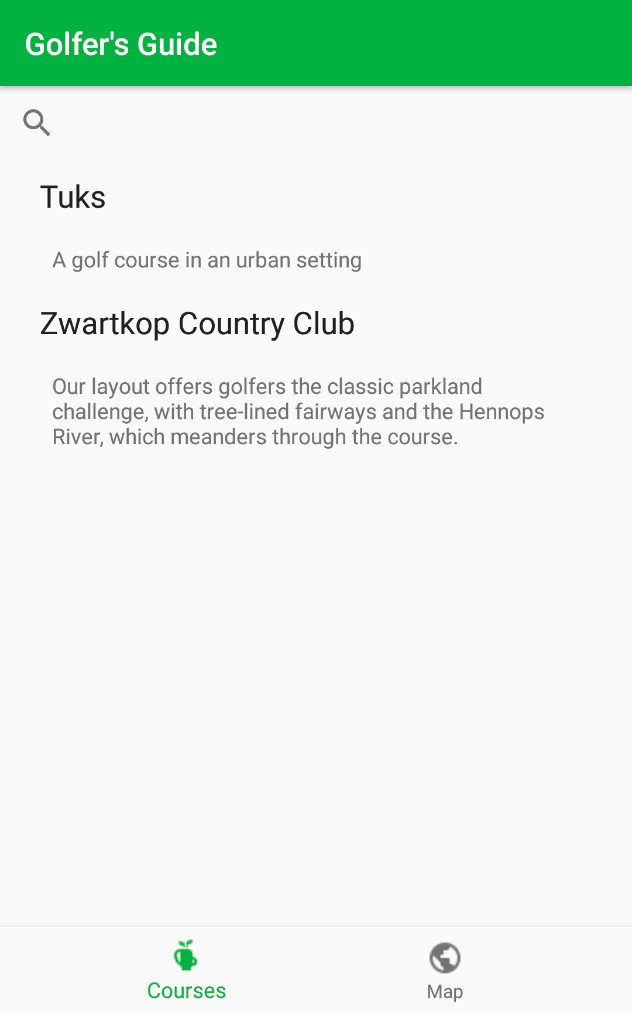
\includegraphics[scale=0.7]{1_courses}
	\paragraph{•}
	Tap on the courses icon at the bottom of the screen see the courses as shown above. There is a search that can be used by pressing on the looking glass icon at the top of the screen.
	
	\subsubsection{Select Hole}
	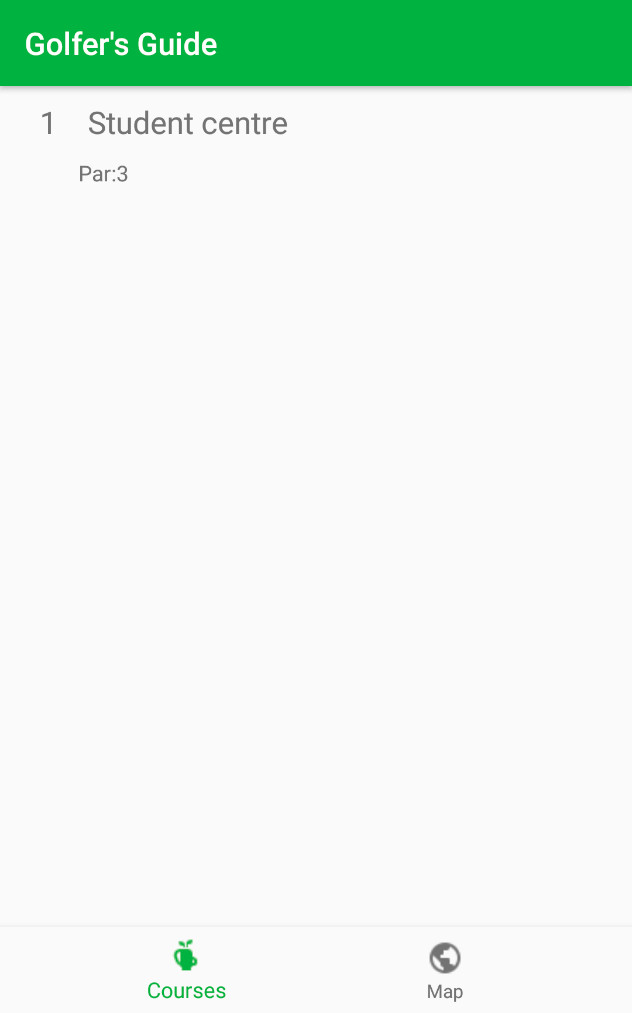
\includegraphics[scale=0.7]{2_holes}
	\paragraph{•}
	After you selected a course, the available holes will be shown as above. Press on the desired hole to load on the map.
	
	\subsubsection{Show Hole}
	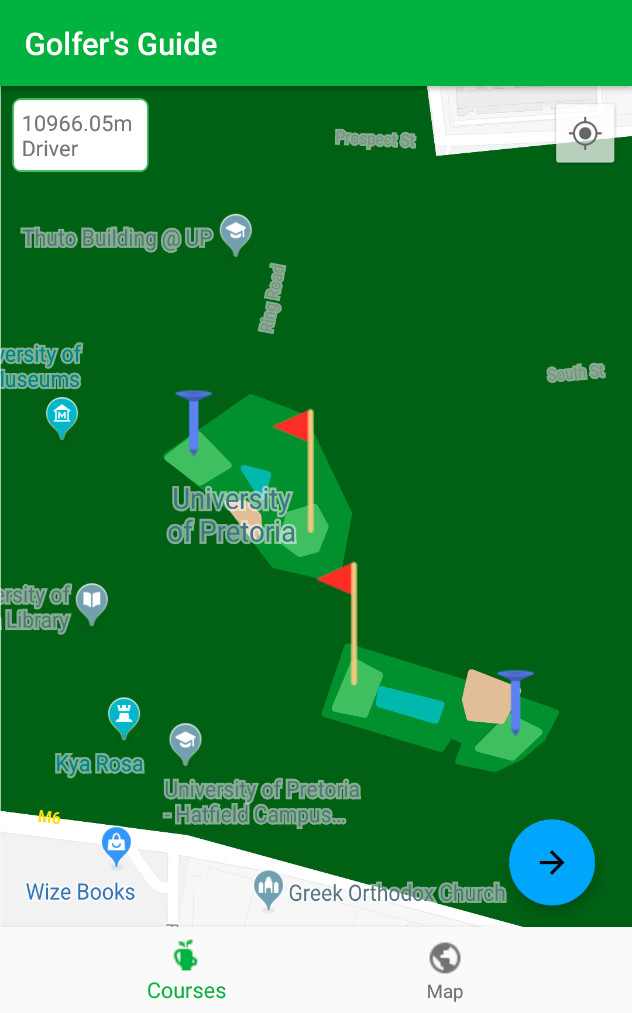
\includegraphics[scale=0.7]{3_course}
	\paragraph{•}
	The map will show the hole on the desired course. 
	
	\subsubsection{Tactical information}
	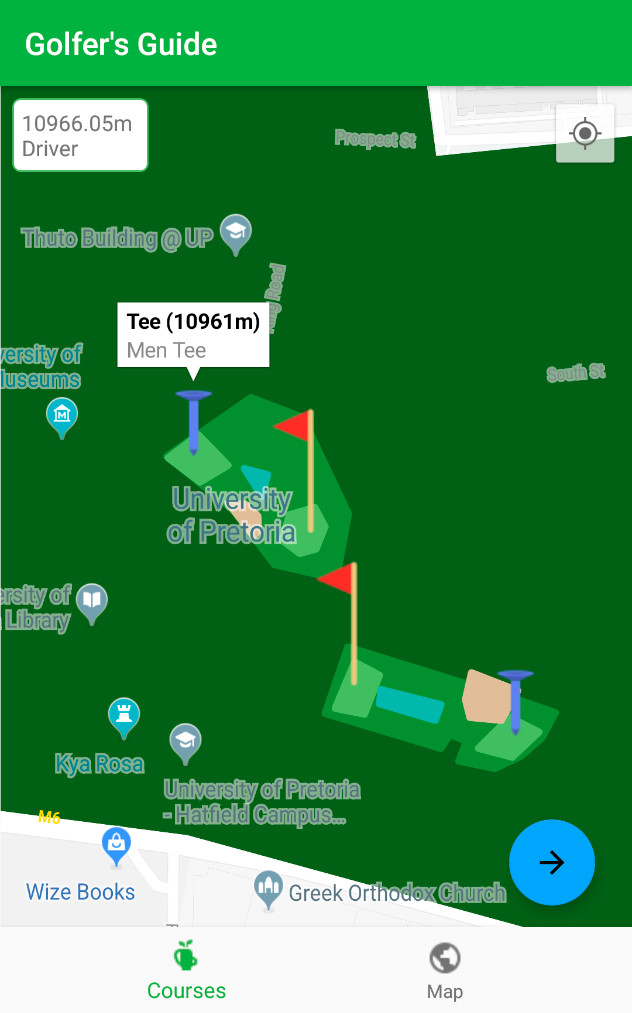
\includegraphics[scale=0.7]{4_info}
	\paragraph{•}
	Tap on any point of interest to see the information about the point and how far the point is away from your current location. In the top right corner, you can also see what golf club is recommended to use.	

	
	\section{Troubleshooting}
	
	Q: The page is not loading.
	\\
	A: Check that you have an internet connection.
	\\
	\\
	Q: The website is giving a random error
	\\
	A: Have you tried turning it off and on again?
	\\
	\\
	Q: The courses are taking too long to load
	\\
	A: The server is under stress, just be patient.
	
	

	
	
\end{document}